\chapter{Background}

This section presents the concepts as well as the original algorithm structure. Dataset examples are provided for each concept. Step-by-step explanations are provided for the algorithm.

% First section: Preliminaries
\section{Preliminaries}

Assuming that we have a dataset that could be presented as a table $T(A_1, A_2, A_3,..A_m, C)$, where $A_{j,m}$ as $1 \leq j \leq m$ are range attributes and $C$ is the categorical class value. A single tuple within $T$ is denoted as $t_k = (v_1,v_2,v_3..v_m,C)$ where $v_m$ is a value under $A_m$.

A sample dataset served as an example for this section can be shown in Table 2.1: 

\begin{table}[h]
\caption{Sample dataset as table}
\label{table:sec1_t1}
\centering
\begin{tabular}{lccccc}
	\toprule
	\textbf{$\mathit{T}$} & \textbf{$\mathit{A_1}$} & \textbf{$\mathit{A_2}$} & \textbf{$\mathit{A_3}$} & \textbf{$\mathit{A_4}$} & \textbf{$\mathit{C}$} \\
	\midrule
	$\mathit{t1}$ & 0.75 & 1.45 & 2.13 & 4.56 & $\mathit{c_1}$ \\
	$\mathit{t2}$ & 0.64 & 1.62 & 2.64 & 4.75 & $\mathit{c_2}$ \\
	$\mathit{t3}$ & 0.71 & 1.21 & 3.11 & 3.97 & $\mathit{c_1}$ \\
	$\mathit{t4}$ & 0.57 & 1.23 & 2.75 & 4.24 & $\mathit{c_1}$ \\
	$\mathit{t5}$ & 0.80 & 1.53 & 2.34 & 4.11 & $\mathit{c_2}$ \\
	\bottomrule
\end{tabular} 
\end{table}
 

\begin{description}

\item[Definition 1 (range)]
Assume within the domain of attribute $A$ exists two values $a$ and $b$ that represent a continuous range over $A_j$, denoted $r = [a,b]_{A_j}$. This range covers a set of values in $A$ that lies between $a$ and $b$. 

\textit{Example 1:} From Table 2.1, a range of $[0.64, 0.75]_{A_1}$ would cover a set of values $0.64$, $0.71$ and $0.75$ in $A_1$.

\item[Definition 2 (cover)]
Assume $r = [a,b]_{A_j}$ to be a range over attribute $A$. This range $r$ covers a set of tuples where their values are between $a$ and $b$ where $a \leq v_j \leq b$. This set of tuples that is covered by $r$ is denoted $\tau(r)$. 

\textit{Example 2:} From Example 1, a range of $[0.64, 0.75]_{A_1}$ would have a cover of tuples $t_2, t_3, t_1$, so its covered tuple set is $t_2, t_3, t_1$.

\item[Definition 3 (associated ranges)]
Assume $r_1 = [a_1,b_1]_{A_1}$ to be a range over $A_1$ and $r_2 = [a_2,b_2]_{A_2}$ to be a range over $A_2$. Those ranges are associated ranges if $\tau(r_1) \cap \tau(r_2) \neq \varnothing$ 

\textit{Example 3:} Assume $r_1 = [0.64, 0.75]_{A_1}$ and $r_2 = [1.21, 1.45]_{A_2}$. Table 2.1 shows that $r_1$ covers $t_1, t_2, t_3$ and $r_2$ covers $t_1, t_4, t_3$, which means $r_1 \cap r_2 = \{t_1, t_2, t_3\} \cap \{t_1, t_3, t_4\} = \{t_1, t_3\}$. Since there are mutual tuples between these ranges, $r_1$ and $r_2$ are associated ranges. 

\item[Definition 4 (range-based classification rule)]
Assume $c$ to be a class value from $C$ and $r_1, r_2, r_3..r_h$ be a set of  associated ranges. $r_1, r_2, r_3..r_h \rightarrow c$ is a range-based classification rule. 

By definition, any tuple $t_k$ can form a rule. However, this will not be accurate nor useful. To determine whether a rule is qualified, there are criteria to be used, which are to be discussed in the sub-section below.

\end{description}

% Second section: Criteria
\section{Criteria}

There are three criteria used in this algorithm: support, confidence and density. This sub-section presents the formal definitions for those measures, while examples are to be provided in the next sub-section where the actual algorithm is reviewed.

\begin{description}
\item[Definition 5 (support)]
Assume $T$ to be a table and $r_1, r_2, r_3..r_h \rightarrow c$ to be a range-based classification rule derived from $T$. The support for $r$, provided $\mid . \mid$ being the size of a set, is: 
\[ \sigma(r) = \frac{\mid \tau(r_1) \cap \tau(r_2) \cap ... \cap \tau(r_h) \mid}{\mid T \mid} \] 

\item[Definition 6 (confidence)]
Assume similar settings from Definition 5, the confidence for $r$  in $T$ is:
\[ \delta(r) = \frac{\mid \tau(r_1) \cap \tau(r_2) \cap ... \cap \tau(r_h) \cap \tau(c) \mid}{\mid \tau(r_1) \cap \tau(r_2) \cap ... \cap \tau(r_h) \mid} \] 

\item[Definition 7 (density)]
Assume similar settings from Definition 5, the density for $r$ in $T$ is:
\[ \gamma(r) = \frac{\mid \tau(r_1) \cap \tau(r_2) \cap ... \cap \tau(r_h) \cap \tau(c) \mid}{\mid \tau(r_1) \cup \tau(r_2) \cup ... \cup \tau(r_h) \mid} \] 

\end{description}


% Section 3: Original Algorithm
\section{Original algorithm}

The original algorithm provides a more efficient way to discover and combine associated ranges for larger rule sets. Instead of traversing through all possible combinations of ranges among all classes and attributes, this algorithm first divides the data into sub-data pools in accordance to its class value. Then, under each attribute, it searches for sub-ranges that could pass certain user-defined thresholds (confidence, support and density). These sub-ranges are then collected and ready to be tested for possible combinations between each other that passes certain thresholds similar to the previous step, which are then collected and ready to be tested for larger combinations. Additionally, after larger combinations are found, an extra adjustment step is done on class values of relevant tuples within the new associated ranges. Afterwards, new associated ranges are ready to be analysed again to find more possible sub-ranges and new combination of sub-ranges. This iteration continues until no possible combinations can be found, so that the last standing associated ranges are translated into the concluding classification rule for that class value. 

To get a clearer structure of the algorithm, its proceedings can be divided into two phases:  

\begin{description}
\item[Phase I (Analyse)] 
This phase has its primary concern as to analyse ranges. Based on the algorithm description, it includes:
	\begin{enumerate}
	\item Partition data into sub-data pool using class values.
	\item For each attribute in sub-data pool, find a maximum and minimum range within that attribute and use it as a starting range for next step.
	\item From min-max starting ranges, search for sub-ranges that passes certain user-specified thresholds such as confidence, support and density. Sub-ranges are collected and passed onto Phase II to generate larger associated ranges.
	\end{enumerate}

\item[Phase II Generate] 
This phase has its primary concern as to generate larger associated ranges for the next iteration. Based on the algorithm, it includes:
	\begin{enumerate}
	\item For each sub-range obtained from last phase, check for possible combination of that range with the remaining ones.
	\item Adjust class values of relevant tuples $r_1, r_2, r_3...r_h \rightarrow c$ under the new combined sub-range.
	\end{enumerate}
\end{description}

Details for each phase are as follows:

\subsection{Original Phase I Analyse}

Given a table $T(A_1, A_2, A_3,..A_m, C)$, the algorithm attemps to seek for classification $r_1, r_2, r_3..r_h \rightarrow c_j$ by finding, among instances that are under class $c_j \in C$, a number of associated ranges $r_1, r_2, r_3..r_h$ that have at least a minimum support ($\sigma_{min}$), density ($\delta_{min}$) and confidence ($\gamma_{min}$) that had previously been specified by the user. This process can be explained in Phase I (Analyse) in which the algorithm seeks for associated ranges and checks if thresholds are satisfied. 

From Figure 2.1, a step-by-step explanation of this algorithm is as follows: 

\begin{figure}[h]
    \centering
    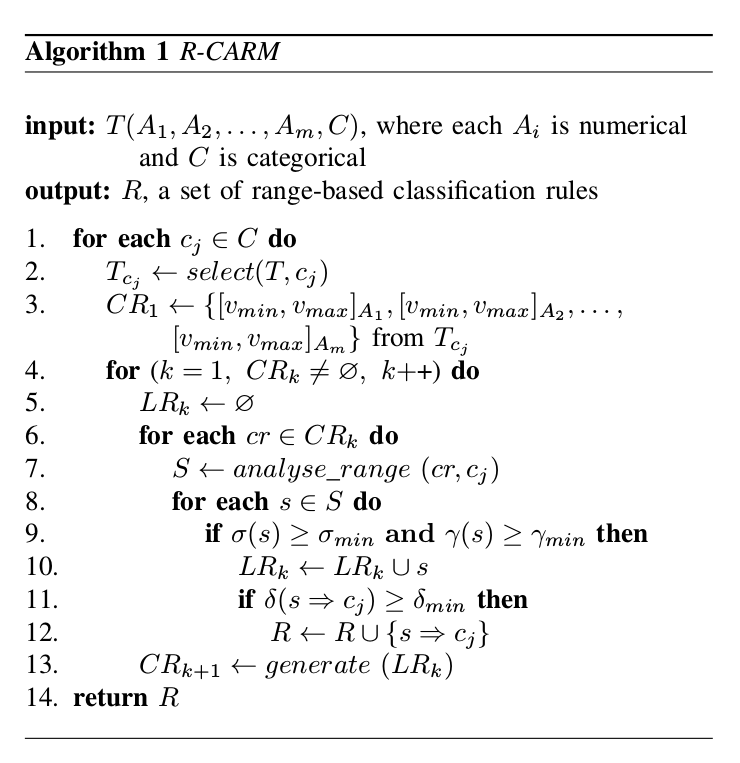
\includegraphics[width=4in]{figures/DrShaoAlgorithm1}
    \caption[Original Phase I Analyse algorithm]{Original Phase I Analyse algorithm}
    \label{fig:figure2_1}
\end{figure}


\begin{description}
\item[Step 1-2] As the beginning steps of the algorithm, they selects a set of tuples $t_1, t_2, t_3..t_N$ from $T$ that has class value $c_j \in C$ and store them in $T_{c_j}$. 

\textit{Example: } Using Table 2.1 from last section, for class $c_j$ where $j$ = 1 (class 1), tuple set $T_{c_1}$ under this class are: 

\begin{table}[h]
\caption{A subset of tuples under class 1}
\label{table:table2_2}
\centering
\begin{tabular}{lccccc}
	\toprule
	\textbf{$\mathit{T_{c_j}}$} & \textbf{$\mathit{A_1}$} & \textbf{$\mathit{A_2}$} & \textbf{$\mathit{A_3}$} & \textbf{$\mathit{A_4}$} & \textbf{$\mathit{C_j}$} \\
	\midrule
	$\mathit{t1}$ & 0.75 & 1.45 & 2.13 & 4.56 & 1 \\
	$\mathit{t3}$ & 0.71 & 1.21 & 3.11 & 3.97 & 1 \\
	$\mathit{t4}$ & 0.57 & 1.23 & 2.75 & 4.24 & 1 \\
	\bottomrule
\end{tabular} 
\end{table}
 

\item[Step 3] In this single step, from $T_{c_j}$, for each attribute $A_i$ the algorithm derives a set of ranges $[v_{min}, v_{max}]_{A_i}$ for that attribute. These ranges are formed by seeking for the minimum and the maximum values of $A_i$ in $T_{c_j}$. This is denoted as candidate ranges $cr$, since they are still subjected to a check to see whether they have the required minimum thresholds needed to form the rules. 

\textit{Example: } From Table 2.2, for each attribute a candidate range can be generated as follows: 
$A_1 = [0.57, 0.75]$, 
$A_2 = [1.21, 1.45]$, 
$A_3 = [2.13, 3.11]$,
$A_4 = [3.97, 4.24]$.

\item[Step 4-13] In these remaining steps lie the core analysis of Phase I, which could be separated into three main components: sub-range derivation, threshold check and larger range generation. Firstly, for each range in $cr$, an analysis is performed to derive possible sub ranges from this range. The reason for this analysis is because for continuous ranges, $[v_{min}, v_{max}]_{A_i}$ could cover more than necessary tuples that consequently reduces the rule accuracy if not trimmed down.
 
\textit{Example: } Consider the example $A_1 = [0.57, 0.75]$ from the previous step. Using this range on the original set of tuples $T$ in Table 2.1, the tuples that the range covers are: 

\begin{table}[h]
\caption{Subset of tuples under class 1 and range r of attribute 1}
\label{table:table2_3}
\centering
\begin{tabular}{lcc}
	\toprule
	\textbf{$\mathit{T}$} & \textbf{$\mathit{A_1}$}   & \textbf{$\mathit{C}$} \\
	\midrule
	$\mathit{t1}$ & 0.75 & 1 \\
	$\mathit{t2}$ & 0.64 & 2 \\
	$\mathit{t3}$ & 0.71 & 1 \\
	$\mathit{t4}$ & 0.57 & 1 \\
	\bottomrule
\end{tabular} 
\end{table}


Under this range $A_1 = [0.57, 0.75]$ which is a candidate rule, its cover of ${t_1,t_2,t_3,t_4}$ gives a $\frac{3}{4}$ correct classification. However, by adjusting the range to $A_1 = [0.68, 0.75]$ which covers ${t_1,t_3,t_4}$, it now gives $\frac{4}{4}$ correct classification. Although the support for this range is reduced, higher classification accuracy is achieved. This adjustment step lies within step 7. 

\item[Step 7] The pruning process is represented by the $analyse\_range$ function, where a method is implemented to find sub-ranges. This method is based on the solution to the max sum problem [SRC], which is for finding a maximal gained sub-array within a given array of discrete numbers (its details will be discussed further in the next section). To apply the similar approach to finding maximum sub-ranges, for class $c_j$, each tuple in $T_{c_j}$ that is covered by range $[v_{min}, v_{max}]_{A_i}$ is scored with $1$ if its class is $c_j$ and $-1$ otherwise. This is to convert continuous values into discrete (in this case, binary) scores of numbers, that are then used to calculate the max sum scores. Those max sum scores represents the candidate sub-ranges, which could be the desired sub-ranges once they satisfy the support confidence and density constraints. There can be multiple sub-ranges and thus all sub-ranges are collected and store the result in set $S$. Sub-ranges in set $S$ is checked in the following step 8-12 for threshold requirements. 

\textit{Example: } From Table 2.3, $T_{A_1}$ where $A_1 = [0.57, 0.75]$ and the class value $c_1$ is $1$, the tuples ${t_1,t_2,t_3,t_4}$ are covered under this rule and can be presented in ascending order as: 
\begin{table}[h]
\caption{A subset analysed by max-sum method for sub-ranges}
\label{table:table2_4}
\centering
\begin{tabular}{lcccc}
	\toprule
	\textbf{} & \textbf{$\mathit{t_2}$}   & \textbf{$\mathit{t_4}$} & \textbf{$\mathit{t_3}$} & \textbf{$\mathit{t_1}$} \\
	\midrule
	Attribute value & 0.64 & 0.68 & 0.71 & 0.75 \\
	Class value & ${c_2}$ & ${c_1}$ & ${c_1}$ & ${c_1}$ \\
	Binary values & -1 & 1 & 1 & 1 \\
	\bottomrule
\end{tabular} 
\end{table}


Assume the max-sum approach requires 100\% confidence i.e. correct classification ($c$ = 1) for each covered tuple, the resulted optimal binary array will be ${ 1 1 1 }$ which represents a sub-range $s = [0.68, 0.75]$ that covers tuples ${t_4,t_3,t_1}$.

\item[Step 8-10] These steps perform a support and density threshold check on sub-ranges in set $S$. For each sub-range $s$ in $S$, a threshold check is performed to see whether it has sufficient support and density specified (Step 9). If sub-range $s$ does, it is kept in $LR_k$ where candidate sub-ranges are stored to form larger associated ranges in the next iteration (Step 10). However, if it does not satisfy the specified thresholds, sub-range $s$ is discarded as it cannot be used to form larger associated ranges due to support and density measures being monotonic \cite{monotonic}. All checked ranges $s$ in $LR_k$ are then passed on for a final check on confidence threshold in the following step 11-13.
 
\textit{Example: } From Table 2.4 where sub-range $s = [0.68,0.75]_{A_1}$ is found for attribute $A_1$, the support and density can be computed as follows:
\[ \sigma_s = \frac{\{t_3,t_4,t_1\}}{\{t_2,t_4,t_3,t_1\}}\ = \frac{3}{4} = 0.75 \] 
\[ \gamma_s = 1 \] 
Assume the condition specified is $\sigma_s \geq 0.6$ and $\gamma_s \geq 0.9$, then sub-range $s = [0.68,0.75]_{A_1}$ satisfies the required support and density threshold and therefore accepted.  
Assume, with the similar rule, another sub-range $s = [1.21, 1.45]_{A_2}$ is found for attribute $A_2$ from an initial range $[1.21, 1.45]_{A_2}$. The support and density can be computed as follows:
\[ \sigma_s = \frac{\{t_3,t_4,t_1\}}{\{t_3,t_4,t_1,t_5,t_2\}}\ = \frac{3}{4} = 0.75 \] 
\[ \gamma_s = 1 \] 
With the same support and density measures, sub-range  $s = [1.21, 1.45]_{A_2}$ is also accepted.
These two sub-ranges are stored in $LR_k$ for the next steps, hence $LR_k = \{[0.68, 0.75]_{A_1}, [1.21,1.64]_{A_2}\}$. \\

\item[Step 11-12] These steps perform the last check for confidence threshold on ranges in $LR_k$. Using class value $c_j$, it checks whether sub-range $s$ in $LR_k$ can be used to form range-based classification rules with sufficient confidence (Step 11-12). If $s$ satisfies the confidence test, sub-range $s$ is then kept in $LR_k$ which is then used to form larger association of ranges. The process of forming larger associated ranges is in Phase II (Generate) in Step 13. However, in cases where $s$ fails to pass the confidence threshold, it is discarded and no longer considered in the next iteration.

\textit{Example: } In Step 8-10 example, sub-range $s = [0.68,0.75]_{A_1}$ is shown to have passed threshold for support and density. It is then checked for confidence measure, which is as follows:
\[ \delta_s = \frac{\{t_4,t_3,t_1\}}{\{t_4,t_3,t_1\}}\ = 1 \] 
Assume the condition specified is $\delta_s \geq 0.8$, sub-range $s = [0.68,0.75]_{A_1}$ passes the test and therefore accepted.
Similarly for sub-range $s = [1.21, 1.45]_{A_2}$:
\[ \delta_s = \frac{\{t_3,t_4,t_1\}}{\{t_3,t_4,t_1\}}\ = 1 \] 
Hence $LR_k = \{[0.68, 0.75]_{A_1}, [1.21,1.64]_{A_2}\}$ is accepted and passed onto Phase II (Generate) in Step 13 to form larger associated ranges.

\item[Step 13] This step, which represents Phase II (Generate), perform the generation of larger associations of ranges $CR_{k+1}$ by a generate function. The process is the core in Phase II (Generate) is described in Phase II sub-section below.

\end{description}

\subsection{Original Phase II Generate}
In this phase, the algorithm prepares $CR_{k+1}$ for the next iteration by combining two relevant ranges in $LR_k$, thus extending the current ranges. The combining process mirrors the A-priori algorithm in generating frequent itemsets in association rule mining. Although A-priori applies on categorical values, it is adapted to this range-based classfication algorithm by using an additional step on range adjustment. The algorithm is denoted in Figure 2.2 below: 

\begin{figure}[h]
    \centering
    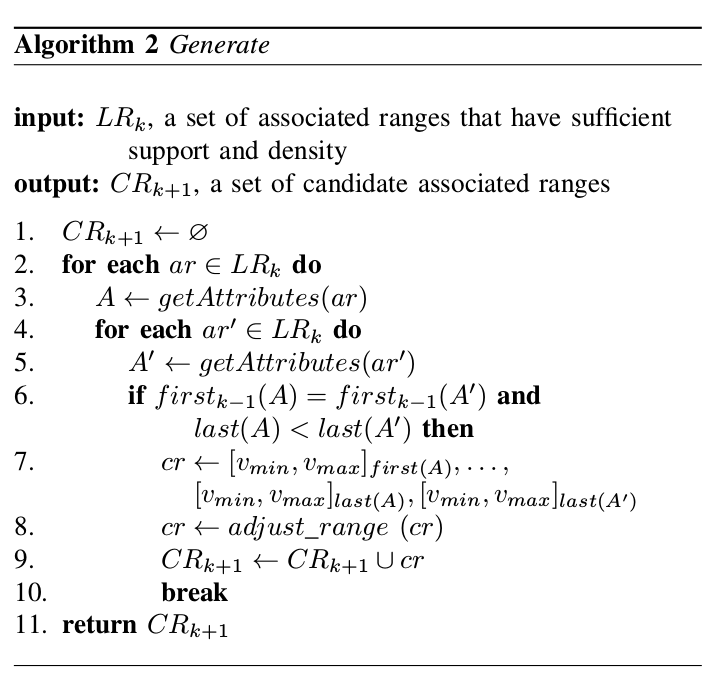
\includegraphics[width=4in]{figures/DrShaoAlgorithm2}
    \caption[Original Phase II Generate algorithm]{Original Phase II Generate algorithm}
    \label{fig:figure2_2}
\end{figure}

\begin{description}
\item[Step 1-5] Given $LR_k$ from previous phase, these steps traverses through all sets of associated ranges in $LR_k$ and for each set of associated ranges $ar$, it looks for another remaining set $ar’$ as a possible set to combine to make a larger range. The condition to combine is in the following Step 6-7. 

\item[Step 6-7] These steps decide whether $ar$ and $ar’$ can be combined by searching whether $ar$ and $ar’$ differs by only one last attribute. $first_{k-1}$ is a function to retrieve the first attribute in each set, and $last$ is a function to retrieve the last attribute in the same set. So if the last function of $ar’$ returns an attribute that is larger than the that which is returned by the last function of $ar$, this pair is accepted. A new extended set of associated range is formed based on this pair, in which the starting range is the same $first_{k-1}$ range and the ending range is the larger $last$ range between the two ranges (Step 7). 

\textit{Example: } From Phase I example, $LR_k = \{[0.68, 0.75]_{A_1}, [1.21,1.64]_{A_2}\}$ is found. Assume another $LR_k = \{[0.68, 0.75]_{A_1}, [2.75,3.11]_{A_3}\}$ is found. A pair between these $LRs$ can be formed since $A_1 = A_1$ and $A_3 > A_2$. A new extended set of assciated ranges $cr$ is
$cr = \{[0.68, 0.75]_{A_1}, [1.21,1.64]_{A_2}, [2.75,3.11]_{A_3}\}$

However, before this set is passed onto the next iteration, an adjustment is necessary since similar issue is encountered from Phase I : A combination of two continuous ranges may cover more than necessary set of tuples. It occurs when a tuple might be covered in range 1, but not covered in range 2 and vice versa. As the new extended set is passed onto the next iteration, those tuples that fail to be covered in all specified ranges shall be set aside. In this algorithm, the algorithm preserves a strict policy of selection: it presumes those tuples would produce wrong classification at the end, thus will change their classes to $Null$ which signifies a possible eliminiation on the next iteration (recall maxsum process in Phase I where it might eliminates tuples that are not under the same class value to trim down the candidate range).

\textit{Example: } An extended set of associated ranges $cr = \{[0.68, 0.75]_{A_1}, [1.21,1.64]_{A_2}, [2.75,3.11]_{A_3}\}$ is found from the last step. This set $cr$ covers tuples under $A_1, A_2, A_3$ respectively as:

\[ cr = \{[0.68, 0.75]_{A_1}, [1.21,1.64]_{A_2}, [2.75,3.11]_{A_3}\} \] 
\[ \{t_4,t_3,t_1\} { } \{t_3,t_4,t_1\} { } \{t_4, t_3\} \] 

It can be seen that tuple $t_1$ is not covered under $A_3$ range.Initially, $t_1$ has class $c_1$, but since it was not covered completely under this set, the algorithm will convert $c_1$ to $Null$ in $t_1$. From Table 2.1, $t_1$ is now presented as: 

\begin{table}[h]
\caption{Tuple turned Null in class value during Generate phase}
\label{table:table2_5}
\centering
\begin{tabular}{lccccc}
	\toprule
	\textbf{$\mathit{T_{c_j}}$} & \textbf{$\mathit{A_1}$} & \textbf{$\mathit{A_2}$} & \textbf{$\mathit{A_3}$} & \textbf{$\mathit{A_4}$} & \textbf{$\mathit{C_j}$} \\
	\midrule
	$\mathit{t1}$ & 0.75 & 1.45 & 2.13 & 4.56 & Null \\
	\bottomrule
\end{tabular} 
\end{table}


Its class will be kept for all iterations under class $c_1$. 

Once Phase II (Generate) is completed, it repeats Phase I (Analyse) but on the new extended set of associated ranges instead. The iteration continues until no possible pair can be formed, which is when the algorithm is concluded. The remaining pair become the classification rule for that class. 

However, it must be noted that this null-class converting process is replaced in this project algorithm, as this project adopts a stricter policy that eliminates partly-covered tuples instead of leaving it for consideration in the next iteration. Explanation and reasoning for such approach is discussed in the next section where the project algorithm is reviewed.

\end{description}
















